\documentclass[10pt,ignorenonframetext,]{beamer}
\setbeamertemplate{caption}[numbered]
\setbeamertemplate{caption label separator}{: }
\setbeamercolor{caption name}{fg=normal text.fg}
\beamertemplatenavigationsymbolsempty
\usepackage{lmodern}
\usepackage{amssymb,amsmath}
\usepackage{ifxetex,ifluatex}
\usepackage{fixltx2e} % provides \textsubscript
\ifnum 0\ifxetex 1\fi\ifluatex 1\fi=0 % if pdftex
  \usepackage[T1]{fontenc}
  \usepackage[utf8]{inputenc}
\else % if luatex or xelatex
  \ifxetex
    \usepackage{mathspec}
  \else
    \usepackage{fontspec}
  \fi
  \defaultfontfeatures{Ligatures=TeX,Scale=MatchLowercase}
\fi
% use upquote if available, for straight quotes in verbatim environments
\IfFileExists{upquote.sty}{\usepackage{upquote}}{}
% use microtype if available
\IfFileExists{microtype.sty}{%
\usepackage{microtype}
\UseMicrotypeSet[protrusion]{basicmath} % disable protrusion for tt fonts
}{}
\newif\ifbibliography
\hypersetup{
            pdftitle={Supporting Data-Intensive Research in the Environmental Sciences},
            pdfauthor={Advisor: Dr.~Stacey Hancock},
            pdfborder={0 0 0},
            breaklinks=true}
\urlstyle{same}  % don't use monospace font for urls

% Prevent slide breaks in the middle of a paragraph:
\widowpenalties 1 10000
\raggedbottom

\AtBeginPart{
  \let\insertpartnumber\relax
  \let\partname\relax
  \frame{\partpage}
}
\AtBeginSection{
  \ifbibliography
  \else
    \let\insertsectionnumber\relax
    \let\sectionname\relax
    \frame{\sectionpage}
  \fi
}
\AtBeginSubsection{
  \let\insertsubsectionnumber\relax
  \let\subsectionname\relax
  \frame{\subsectionpage}
}

\setlength{\parindent}{0pt}
\setlength{\parskip}{6pt plus 2pt minus 1pt}
\setlength{\emergencystretch}{3em}  % prevent overfull lines
\providecommand{\tightlist}{%
  \setlength{\itemsep}{0pt}\setlength{\parskip}{0pt}}
\setcounter{secnumdepth}{0}
\usepackage{float} \usepackage{bm} \usepackage{amsmath}
\usepackage{amssymb} \usepackage{multicol} \usepackage{tikz}
\usepackage{graphicx}

\title{Supporting Data-Intensive Research in the Environmental Sciences}
\subtitle{Allison Theobold}
\author{Advisor: Dr.~Stacey Hancock}
\date{October 10, 2018}

\begin{document}
\frame{\titlepage}

\begin{frame}{Outline}

\begin{itemize}[<+->]
\tightlist
\item
  Study Motivation\\
\item
  Research Questions\\
\item
  Pilot Study \& Faculty Interviews\\
\item
  Study Design for Workshops\\
\item
  Data Collection \& Analysis\\
\item
  Benefits of Research
\end{itemize}

\end{frame}

\begin{frame}{A Motivating Vignette}

\begin{itemize}[<+->]
\item
  Suppose you are an Ecology graduate student studying the abundance of
  wild and hatchery-raised pallid sturgeon. You have collected data over
  the last 2 years on fish abundance along the same reaches of the
  Missouri River, to look for trends in fish abundance.
\item
  When recording your data in Excel, you chose for each section of the
  Missouri to be a row and every sampling instance to be a different
  column.
\end{itemize}

\end{frame}

\begin{frame}[fragile]{Data Problems}

\begin{multicol}{2}





\end{multicol}

\begin{itemize}[<+->]
\tightlist
\item
  The \texttt{R} functions you saw in your courses require for your data
  to be in long format.
\end{itemize}

\begin{itemize}[<+->]
\tightlist
\item
  What would you do? Where would you go for help?
\end{itemize}

\end{frame}

\begin{frame}{Motivation}

\begin{itemize}[<+->]
\item
  Changing practice of environmental science has changed, because of
  growth in computational power and the volume and variety of available
  data.
\item
  Applications of statistical approaches that rely on computation, such
  as big data management, dynamic data visualization, and simulation
  based analyses, have become essential understandings for field
  applications (Weintrop et al., 2016).
\item
  These advances have created a growing need for scientists to receive
  an appropriate education in computational methods and techniques
  relevant to their discipline.
\item
  The growing need for computation in science education is greater than
  ever (Fox \& Ouellette, 2013).
\end{itemize}

\end{frame}

\begin{frame}{(Lack of) Computing in Environmental Sciences}

\begin{itemize}[<+->]
\item
  In this rapidly changing computational landscape calls have surfaced
  to re-evaluate how curricula to ``better prepare current and future
  generations of environmental researchers'' (Green et al., 2005;
  Hampton et al., 2016).
\item
  Over the last twenty years, Statistics preparation in the
  environmental sciences has become vital.

  \begin{itemize}[<+->]
  \tightlist
  \item
    Hence, Statistics courses have been incorporated into these graduate
    programs, across the nation.
  \end{itemize}
\end{itemize}

\end{frame}

\begin{frame}{(Lack of) Computing in Environmental Sciences}

\begin{itemize}[<+->]
\tightlist
\item
  A 2012 survey of graduate students:

  \begin{itemize}[<+->]
  \tightlist
  \item
    over 80\% of students reported that they had received no formal
    training in computing, even at the most basic level\\
  \item
    74\% stated that they had no skills in any programming language
    (Hernandez, Meyernik, Murphy-Mariscal \& Allen, 2012).
  \end{itemize}
\item
  And most, if not all of what is known about data management,
  visualization, and analysis has been learned piecemeal, or not learned
  at all (Teal et al., 2015).
\end{itemize}

\end{frame}

\begin{frame}{Why Aren't They Learning Computing?}

\begin{itemize}[<+->]
\item
  ``What we teach {[}in Statistics{]} lags decades behind what we
  practice'' and ``the gap between our half-century-old curriculum and
  our contemporary statistical practice continues to widen'' (Cobb,
  2015).
\item
  ``Computing has been one of the most glaring omissions in the set of
  tools that have so far defined Statistics education'' (Friedman,
  2001).
\item
  In our courses, do students build the confidence needed to overcome
  computational challenges?
\end{itemize}

\end{frame}

\begin{frame}{What Do We Teach?}

\begin{itemize}[<+->]
\item
  ``Most of our students are not prepared for data analysis after their
  statistics {[}courses{]},'' because ``they have done very little
  actual data analysis'' (Nolan \& Temple Lang, 2010).\\
\item
  Lumley (2015) stated that our students know how to deal with
  \(n \to \infty\) but cannot deal with a million observations.
\item
  Students are either ``told to learn how to program by themselves, from
  each other, or from their teaching assistant in a two-week''crash
  course" at the start of a course."

  \begin{itemize}[<+->]
  \tightlist
  \item
    Sends a signal to students that computing is not of intellectual
    importance (Nolan \& Temple Lang, 2010)
  \end{itemize}
\end{itemize}

\end{frame}

\begin{frame}{Barriers to Incorporating Computing}

\begin{itemize}[<+->]
\item
  Attempting to fit more material into already-full courses and
  curricula.
\item
  Potentially taught by people who may not feel prepared teach these
  topics.
\item
  Not clear what computing should be included and how.
\item
  Not all institutions have the flexibility to develop a statistics
  course on computing with data.
\end{itemize}

\end{frame}

\begin{frame}{Computational Knowledge Acquisition}

\begin{itemize}[<+->]
\item
  Most researchers ``learn what they know about programming and data
  management on their own or the information is passed down within a
  lab'' (Teal et al, 2015).
\item
  This process results in substantial hidden costs:

  \begin{itemize}[<+->]
  \tightlist
  \item
    students pick up bad habits and misunderstandings\\
  \item
    learn just enough to get through\\
  \item
    initial knowledge severely limits them
  \end{itemize}
\end{itemize}

\end{frame}

\begin{frame}{The Lens of Distributed Cognition}

\begin{itemize}[<+->]
\tightlist
\item
  Investigates the organization of cognitive systems but differs
  substantially from traditional cognitive theory.

  \begin{itemize}[<+->]
  \tightlist
  \item
    Considers systems beyond the individual.
  \item
    Includes interactions between individuals.
  \item
    Incorporates resources and materials into an individual's
    environment.
  \end{itemize}
\item
  These resources are shared socially to extend an individual's ability
  to accomplish something that they otherwise could not achieve alone.
\end{itemize}

\end{frame}

\begin{frame}{Beliefs of Distributed Cognition}

\begin{itemize}[<+->]
\item
  Individuals coordinate different types of structure in their
  environment.
\item
  Coordinating these different structures requires effort.
\item
  Individuals off-load tasks with high cognitive effort to their
  environment, whenever possible.
\item
  Dynamics of cognitive load-balancing are available through social
  organizations.
\end{itemize}

\end{frame}

\begin{frame}{Research Questions}

\begin{enumerate}[<+->]
\def\labelenumi{\arabic{enumi}.}
\item
  What computing skills are necessary for environmental science graduate
  students to successfully implement applications of statistics in their
  research?
\item
  How are students filling the gap between the computing skills they
  know and the computing skills they need to know, in order to perform
  applications of statistics in their research?
\item
  How can workshops help to alleviate this gap between statistical
  computing preparation and expectations?
\end{enumerate}

\end{frame}

\begin{frame}{Pilot Study (Spring 2017)}

\begin{itemize}[<+->]
\tightlist
\item
  In my pilot study we asked environmental science graduate students to
  complete applications of statistical computing, in the context of
  ecological data.
\end{itemize}

\begin{center}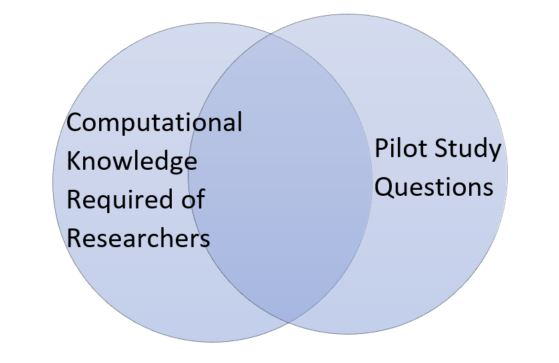
\includegraphics[width=600px]{PilotQuestions} \end{center}

\end{frame}

\begin{frame}{Paths for Acquisition of Statistical Computing Skills}

\begin{center}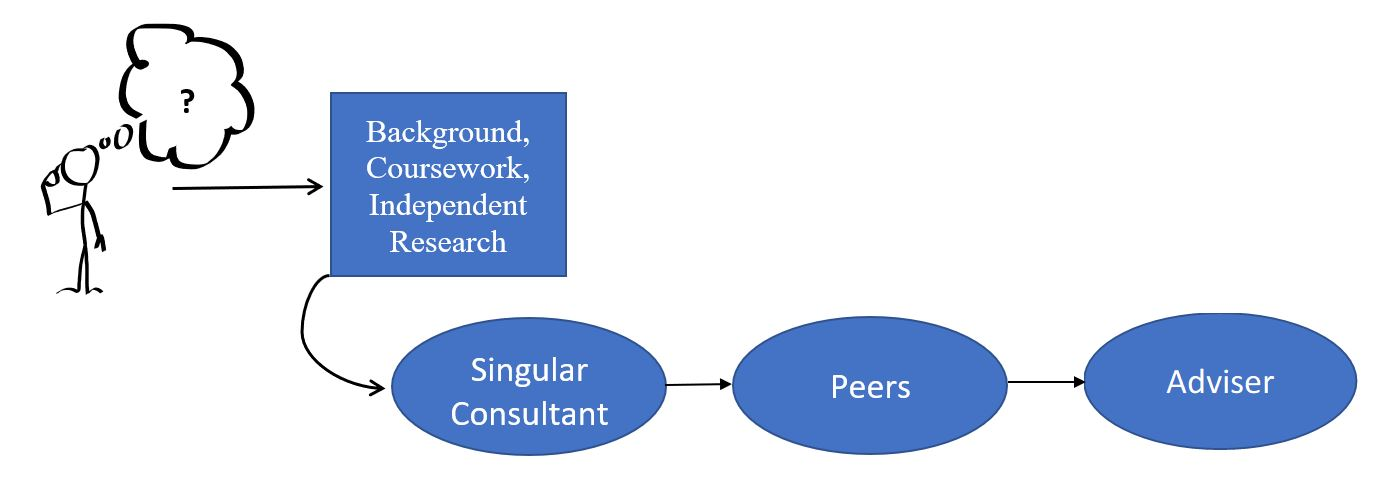
\includegraphics[width=800px]{Path} \end{center}

\end{frame}

\begin{frame}{Faculty Interviews (Spring 2018)}

\begin{itemize}[<+->]
\item
  Montana State faculty attributed these gaps in students' computational
  preparation, to the computational curricula at a university being
  driven by its faculty.

  \begin{itemize}[<+->]
  \tightlist
  \item
    \emph{``Most graduate students come in knowing more about the tools
    one would use to manipulate data than their advisors do, at this
    point.''}\\
  \item
    \emph{``I think the expectations have gone up in order of magnitude
    in the last decade. We have very high expectations of statistics and
    very low expectations in computation.''}
  \item
    \emph{``We had a computer science Python course that I took my first
    semester in grad school. That semester, I realized that
    {[}computing{]} was where biology was going.''}
  \end{itemize}
\end{itemize}

\end{frame}

\begin{frame}{Gaps in Computational Preparation}

\begin{itemize}[<+->]
\tightlist
\item
  Computational understandings from Statistics coursework, were
  primarily low-level concepts.

  \begin{itemize}[<+->]
  \tightlist
  \item
    \emph{``By the end of the semester I wouldn't look at what the code
    was doing, I would just run it.''}\\
  \item
    \emph{``I had to learn the R first and then I could look back at the
    code and understand what was going on.''}
  \end{itemize}
\item
  Understandings informed by a student's independent research, were
  described largely as high-level concepts.

  \begin{itemize}[<+->]
  \tightlist
  \item
    \emph{``The data management stuff comes from independent research,
    trial and error, getting myself through.''}
  \end{itemize}
\end{itemize}

\vspace{2cm}

\begin{itemize}[<+->]
\tightlist
\item
  \textbf{Proposed Solution:} workshops to develop computing skills
\end{itemize}

\end{frame}

\begin{frame}{Computing Learning Trajectory}

\vspace{4cm}

\begin{center}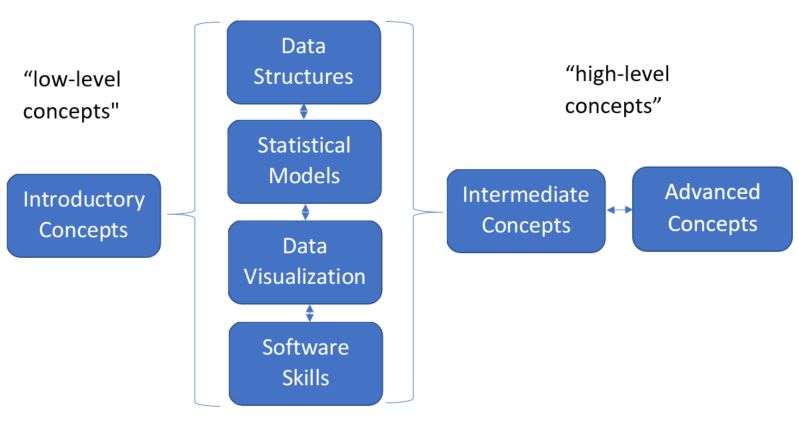
\includegraphics[width=800px,height=350px]{Trajectory2} \end{center}

\begin{itemize}[<+->]
\tightlist
\item
  ``Instead of learning some things here and there, programming is a
  skill that is learned by building new information on top of earlier
  information'' (Fuller et al., 2007).
\end{itemize}

\end{frame}

\begin{frame}{Classroom (Workshop) Design Study}

\begin{itemize}[<+->]
\item
  Systematically study the development of computational skills, in the
  context of environmental science research.
\item
  Including the design of a means by which to support the development of
  these computational skills.

  \begin{itemize}[<+->]
  \tightlist
  \item
    investigate how to support this learning
  \item
    develop, test, and revise conjectures about the learning process and
    how to support that learning
  \end{itemize}
\end{itemize}

\vspace{1cm}

\begin{itemize}[<+->]
\tightlist
\item
  A design study is appropriate because:

  \begin{itemize}[<+->]
  \tightlist
  \item
    it is difficult to study the learning of computing skills by
    observation\\
  \item
    current research does not formulate what computational skills are
    necessary and how to be teach them
  \end{itemize}
\end{itemize}

\end{frame}

\begin{frame}{Components of a Design Study}

\begin{itemize}[<+->]
\item
  Specify goals for students' learning
\item
  Document workshop starting points
\item
  Delineate an envisioned learning trajectory
\item
  Place the study in a theoretical context
\item
  Iterate between workshop design, data collection, and analysis
\end{itemize}

\end{frame}

\begin{frame}{Workshop Learning Goals}

\begin{itemize}[<+->]
\item
  Unreasonable to expect that every researcher is an expert in their
  domain science, Statistics, data management, processing, and
  visualization (Hampton et al., 2015, p.~547).
\item
  Researchers should have the computational tools to:

  \begin{itemize}[<+->]
  \tightlist
  \item
    work with messy or organized datasets, stored in varied data
    formats, in a reproducible workflow\\
  \item
    employ a variety of statistical methods and simulation\\
  \item
    make use of basic software skills\\
  \item
    create effective data visualizations (Hampton et al., 2015, p.~547)
  \end{itemize}
\end{itemize}

\end{frame}

\begin{frame}[fragile]{Workshop Structure - Starting Points}

\begin{itemize}[<+->]
\item
  In reasoning through computational problems, students' misconceptions
  of foundational concepts became unveiled.
\item
  \textbf{Example:} Many misunderstandings revolved around how
  \texttt{R} interprets logicals (TRUE/FALSE).

  \begin{itemize}[<+->]
  \tightlist
  \item
    \emph{``Using the subset command where you call the data fame and
    you have your {[}{]}, and just do -c(species =
    c(''Bull``,''WCT``)).''}\\
  \item
    \emph{``I think you can remove observations by putting the
    observation number, but I don't know exactly how.''}
  \item
    \emph{``I didn't know that was what was going on {[}subset using
    logicals{]}. I don't know if I was ever taught that.''}
  \end{itemize}
\end{itemize}

\end{frame}

\begin{frame}{Workshop Material - Starting Points}

\begin{itemize}[<+->]
\item
  Montana State faculty from environmental science fields were
  interviewed regarding the computational expectations they believed
  were necessary for Master's and Doctoral research in their field.
\item
  Computational expectations varied across fields of research, however,
  many faculty emphasized:

  \begin{itemize}[<+->]
  \tightlist
  \item
    writing functions\\
  \item
    using conditional statements\\
  \item
    looping \& vectorization\\
  \item
    database storage\\
  \item
    data manipulation
  \end{itemize}
\end{itemize}

\end{frame}

\begin{frame}{Computational Skills Data Collection}

\begin{itemize}[<+->]
\tightlist
\item
  A ``control'' cohort of first year environmental science graduate
  students were recruited in Spring 2018 to follow through their program
  of study.

  \begin{itemize}[<+->]
  \tightlist
  \item
    None of the students participated in a workshop.
  \item
    Code generated for research practices.
  \item
    Interviews on acquisition of computational skills.
  \end{itemize}
\end{itemize}

\begin{itemize}[<+->]
\tightlist
\item
  Observations of common environmental science courses which teach
  computing (e.g.~WILD 401, PSPP 516).

  \begin{itemize}[<+->]
  \tightlist
  \item
    Collection of associated course materials (syllabi, labs, online
    resources).
  \end{itemize}
\end{itemize}

\end{frame}

\begin{frame}{(Holistic) Workshop Data Collection}

\begin{itemize}[<+->]
\tightlist
\item
  Prior to the workshop, participants are surveyed for:

  \begin{itemize}[<+->]
  \tightlist
  \item
    demographic information
  \item
    what they expect and want to learn
  \item
    what resources they have used to learn statistical computing
  \end{itemize}
\item
  Additionally, participants are asked to:

  \begin{itemize}[<+->]
  \tightlist
  \item
    provide responses to ``hands-on'' applications of computational
    tasks
  \item
    evaluate workshop effectiveness
  \end{itemize}
\end{itemize}

\end{frame}

\begin{frame}{(Intervention) Workshop Data Collection}

\begin{itemize}[<+->]
\tightlist
\item
  An ``intervention'' cohort of first year graduate students will be
  recruited in spring 2019.

  \begin{itemize}[<+->]
  \tightlist
  \item
    Attend all four workshops in spring 2019.
  \item
    Interview prior to first workshop, for baseline computational
    knowledge.
  \item
    Interview following each workshop, to evaluate workshop environment,
    content, and student learning.
  \item
    Collect and analyze the code generated for research practices.
  \item
    Interviews to investigate acquisition of computational skills.
  \end{itemize}
\end{itemize}

\end{frame}

\begin{frame}{Analytical Framework (Computing Skills)}

\begin{itemize}[<+->]
\tightlist
\item
  Interviews with ``control'' cohort will be transcribed, and
  descriptive coding will be implemented to detail

  \begin{itemize}[<+->]
  \tightlist
  \item
    the computing skills participants employed to use statistics in
    their research\\
  \item
    how they acquired their knowledge of these computational skills
  \end{itemize}
\item
  Course materials will be analyzed to isolate

  \begin{itemize}[<+->]
  \tightlist
  \item
    computing concepts taught\\
  \item
    instructional context used
  \end{itemize}
\item
  Course observations will be transcribed to analyze

  \begin{itemize}[<+->]
  \tightlist
  \item
    nature of classroom discourse\\
  \item
    pedagogical methods of instruction
  \end{itemize}
\end{itemize}

\end{frame}

\begin{frame}{Analytical Framework (Workshops)}

\begin{itemize}[<+->]
\item
  Workshop materials will be kept from fall 2018, to identify

  \begin{itemize}[<+->]
  \tightlist
  \item
    the aspects of the workshop learning environment that evolved over
    the duration of the study
  \end{itemize}
\item
  Interviews with ``intervention'' cohort will be transcribed, and
  descriptive coding will be implemented to detail

  \begin{itemize}[<+->]
  \tightlist
  \item
    the process of students' learning in the workshop sessions
  \item
    aspects of the workshop environment that helped promote learning
  \end{itemize}
\item
  Following each workshop session, debriefing meetings with the
  researchers and assistants will be held.
\item
  Revised learning trajectory for the study, will be created at the
  close of each semester's workshops.
\end{itemize}

\end{frame}

\begin{frame}{Benefits to Environmental Science Research}

\begin{itemize}[<+->]
\item
  Outline key computational skills necessary for successful
  implementation of statistics to research in the environmental
  sciences.
\item
  Detail the paths that students are employing when faced with
  computational challenges for their research.
\item
  Understanding the importance of core skills for data-intensive
  environmental science research will help ``facilitate the integration
  of training into the university'' (Hampton et al., 2015, p.~555).
\end{itemize}

\end{frame}

\begin{frame}{Benefits for Environmental Science \emph{Researchers}}

\begin{itemize}[<+->]
\item
  The materials developed through these workshops will be publicly
  available.
\item
  Create new tools to enhance students' learning of core computational
  skills, necessary for environmental science research.
\item
  Introductory workshops have no barriers to entry. 
\end{itemize}

\end{frame}

\begin{frame}{Benefits to Curriculum}

\begin{itemize}[<+->]
\tightlist
\item
  The pace of technological development can demand that workshops thrive
  outside of university curricula.

  \begin{itemize}[<+->]
  \tightlist
  \item
    Capable of adapting materials rapidly, following computational and
    disciplinary changes.
  \end{itemize}
\item
  Help to ease transition to integrating computing into the
  environmental science and Statistics curricula.

  \begin{itemize}[<+->]
  \tightlist
  \item
    Pooling of resources, so that the materials are available in formats
    that can be quickly adapted and customized.
  \end{itemize}
\end{itemize}

\end{frame}

\begin{frame}{References}

\begin{center}
\includegraphics[width=100px]{RPubs} \end{center}

\url{http://rpubs.com/atheobold/proposal}

\end{frame}

\end{document}
